\pagenumbering{arabic}

\chapter{Introduction} \label{introduction}

For further explanation and details, please, turn to the referred clauses of IEEE 29148-2018, the highlighted and commented version; pay attention to the comments. Clause numbers are written in \textit{italic} in the sections.

Refer to \textit{(Clause 9.6.1)}. 

\section{Purpose of the System }
 Refer to \textit{(Clause 9.6.2, 9.5.2, 9.4.2)}. 

If you want to write unordered (bulleted) lists, you should use an "itemize" environment, where each list entry starts by using the \verb|\item| command, which also generates the bullet symbol.

\begin{itemize}
    \item Item1  
    \item Item2 
\end{itemize}

Numbered lists have the same syntax but use an "enumerate" environment: each entry must be preceded by the \verb|\item|, which will automatically generate numbers to label the item. 

For any citation, refer to it as \cite{younis2021hybrid}.

\section{Scope}

Refer to \textit{(Clause 9.6.3, 9.5.3, 9.4.3)}

\section{System Overview}


\subsection{System Perspective}

\textbf{Context diagram and the explanations of context} go here. Plus, other content as appropriate. This subsection (namely 1.3.1) should be a summary; defer technical details to Section \ref{specificRequirements}. (This was called cross-referring.)

Refer to \textit{(Clause 9.6.4, 9.5.4.1)}
\subsubsection{System Interfaces}
Refer to \textit{(Clause 9.6.4.1)}
\subsubsection{User Interfaces}
Refer to \textit{(Clause 9.6.4.2)}
\subsubsection{Hardware Interfaces}
Refer to \textit{(Clause 9.6.4.3)}
\subsubsection{Software Interfaces}
Refer to \textit{(Clause 9.6.4.4)}
\subsubsection{Communication Interfaces}
Refer to \textit{(Clause 9.6.4.5)}
\subsubsection{Memory Constraints}
Refer to \textit{(Clause 9.6.4.6)}
\subsubsection{Operations}
Refer to \textit{(Clause 9.6.4.7)}

\subsection{System Functions}

Refer to \textit{(Clause 9.6.5, 9.5.4.2)}. If you want to add any figure or diagram, you can use a figure environment.In Figure \ref{Fig:Example}

\begin{figure}[ht]
\centering
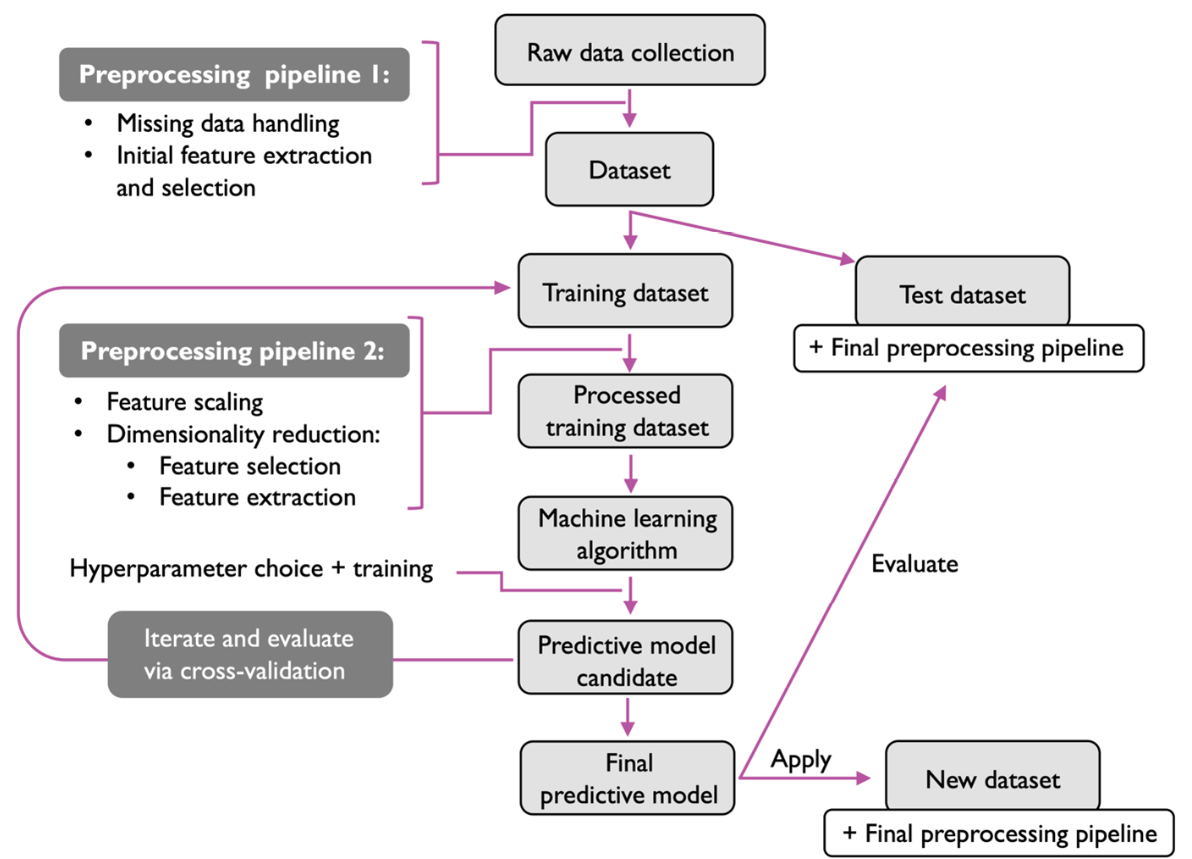
\includegraphics[width=.9 \textwidth]{Figures/ExampleFigure.png}
\caption{Example \label{Fig:Example}}
\end{figure}


\subsection{Stakeholder Characteristics}

Refer to \textit{(Clause 9.6.6, 9.5.4.3, 9.4.5)}

\subsection{Limitations}

Refer to \textit{(Clause 9.6.7)}

\section{Definitions}

You should add acronyms and abbreviations here. Refer to \textit{(Clause 9.6.7)}



For any citation, refer to it as \cite{younis2021hybrid}.
